\documentclass[11pt,a4paper]{article}

% 导言区：加载宏包、设置样式
\usepackage[UTF8]{ctex}      % 中文支持
\usepackage{amsmath,amssymb} % 数学
\usepackage{graphicx}        % 图片
\usepackage{booktabs}        % 三线表
\usepackage{longtable}       % 可跨页的长表格（普通 table 不能跨页）
\usepackage{framed}          % 带边框的纯文本代码框
\usepackage{algorithm}       % 算法浮动体
\usepackage{algpseudocode}   % 伪代码（算法体）排版
\usepackage{hyperref}        % 超链接
\usepackage{geometry}

% 算法环境的标题与输入/输出标签改为中文
\floatname{algorithm}{算法}
\renewcommand{\algorithmicrequire}{\textbf{输入：}}
\renewcommand{\algorithmicensure}{\textbf{输出：}}
\geometry{margin=2.5cm}

% 等宽字体替换为含 Unicode 制表符的字体
\setmonofont{Menlo}[Scale=0.9]

\title{基于传统敏捷与智能AI的软件需求建模对比实验报告}
\author{周溢权}
\date{\today}

% 正文区
\begin{document}
\maketitle
\tableofcontents
\newpage

\section{任务1：传统敏捷人工需求建模（基础）}

\begin{itemize}
    \item 基于原始模糊需求，人工梳理完整业务需求
    \item 完成史诗需求拆分，编写至少8条符合INVEST原则的用户故事
    \item 针对核心业务场景，编写至少3组标准化Gherkin格式BDD行为场景（含正向/异常场景）
\end{itemize}

\subsection{完整业务需求梳理}

\begin{table}[htbp]
    \centering
    \caption{完整业务需求梳理}
    \begin{tabular}{@{}p{0.2\textwidth}p{0.72\textwidth}@{}}
        \toprule
        \textbf{内容} & \textbf{示例} \\
        \midrule
        对象 & 学生、管理员和座位资源 \\
        目标 & 可以更好地管理作为资源，方便学生选座和管理员管理 \\
        学生 & 查看座位空闲时间，进行预约、暂离和释放；学生违约惩罚 \\
        管理员 & 管理座位资源，开放和关闭座位 \\
        座位资源 & 预约、签到和释放 \\
        \bottomrule
    \end{tabular}
\end{table}

\subsection{需求拆分与用户故事}
可以先分成查找座位、预约座位、履约签到等功能，再拆成具体故事：

\begin{framed}
\begin{verbatim}
史诗：管理校园自习室预约
├─ 查找座位
│  ├─ 查看指定时段的空位
│  └─ 按教学楼筛选空位
└─ 预约与履约
   ├─ 预约空闲座位
   ├─ 取消未开始的预约
   ├─ 预约未来扣除信誉分
   ├─ 为预约座位签到
   └─ 暂离和释放
\end{verbatim}
\end{framed}

\begin{table}[htbp]
    \centering
    \caption{用户故事列表}
    \begin{tabular}{@{}p{0.12\textwidth}p{0.8\textwidth}@{}}
        \toprule
        \textbf{编号} & \textbf{用户故事} \\
        \midrule
        US-01 & 作为学生，我想查看指定时段的空闲座位，以便决定去哪里自习。 \\
        \midrule
        US-02 & 作为学生，我想按教学楼筛选空闲座位，以便找到离我较近的位置。 \\
        \midrule
        US-03 & 作为学生，我想预约一个空闲座位，以便到场后有座位可用。 \\
        \midrule
        US-04 & 作为学生，我想取消尚未开始的预约，以便把不用的座位释放给别人。 \\
        \midrule
        US-05 & 作为学生，我想为已预约的座位签到，以便系统确认我已到场。 \\
        \midrule
        US-06 & 作为学生，我想暂时释放座位，以便稍后回来还有座位可用。 \\
        \midrule
        US-07 & 作为管理员，我想设置教室的开放时段，以便阻止学生预约未开放的时段。 \\
        \midrule
        US-08 & 作为管理员，我想在学生自习需求高时增加自习室资源，以便服务更多的学生。 \\
        \midrule
        US-09 & 作为管理员，我想阻止学生预约不来，影响其他同学选座，以便合理分配座位资源。 \\
        \bottomrule
    \end{tabular}
\end{table}

\subsection{Gherkin格式BDD}

\begin{framed}
\begin{verbatim}
Feature: 预约座位

  Scenario: 成功预约空闲座位
    Given 学生已登录，且 A-101 座位在 14:00 至 16:00 空闲
    When 学生预约该座位和时段
    Then 系统生成一条有效预约记录
    And 该座位在该时段变为已预约

  Scenario: 两人同时预约同一个空位
    Given 某时段只剩一个空闲座位
    When 两名学生同时预约该座位
    Then 只有一人的预约成功
    And 系统只生成一条有效预约记录
    And 另一人收到座位已被占用的提示
\end{verbatim}
\end{framed}

\newpage

\begin{framed}
\begin{verbatim}
Feature: 超时未签到释放座位

  Scenario: 超时后释放座位
    Given 学生预约了 14:00 开始的座位，且一直未签到
    When 系统在 14:16 检查该预约
    Then 预约失效，座位重新变为空闲
    And 学生收到超时通知
    And 学生受信誉积分处罚

  Scenario: 已签到的座位不被释放
    Given 学生预约了 14:00 开始的座位，并已在规定时间内签到
    When 系统在 14:16 检查该预约
    Then 预约保持有效
    And 座位不会重新开放预约
\end{verbatim}
\end{framed}

\begin{framed}
\begin{verbatim}
Feature: 管理员新增教室

  Scenario: 成功新增教室
    Given 管理员已登录，且教室编号 A-102 尚不存在
    When 管理员提交 A-102 的教室及座位信息
    Then 教室列表显示 A-102
    And 学生可以查询其开放时段的座位

  Scenario: 拒绝重复的教室编号
    Given 系统中已经存在教室 A-102
    When 管理员再次提交编号为 A-102 的教室
    Then 系统提示编号已存在
    And 教室列表中仍只有一个 A-102
\end{verbatim}
\end{framed}

\section{任务2：LLM增强需求建模（进阶）}

\begin{itemize}
    \item 设计合理Prompt，基于同一原始需求，通过大模型完成需求结构化梳理
    \item AI生成用户故事与BDD场景，对比人工版本，完成修正、去重、补全
    \item 总结LLM在需求建模中的优势与存在的缺陷（幻觉、场景冗余、逻辑偏差等）
\end{itemize}

\subsection{Prompt 设计与对话记录}

\begin{itemize}
    \item \textbf{使用模型}：DeepSeek V4.1 Flash（网页端）
    \item \textbf{对话记录}：\href{https://chat.deepseek.com/share/yctx43ujc0k2kh6jxo}{DeepSeek 对话分享链接}
\end{itemize}

\noindent\textbf{Prompt}：

\begin{framed}
\noindent 你是一个专业的软件工程专家，有着丰富的软件开发工程经验。现在需要开发一个「校园自习室智能预约系统」，我需要你给出此系统设计的需求结构化梳理，生成用户故事和 Gherkin 格式的 BDD 场景。
\end{framed}

\subsection{AI生成的用户故事（节选）}
LLM 共生成 20 条用户故事，覆盖登录、查询、预约、签到、资源管理与安全，并扩展到智能推荐、候补和信用治理。表~\ref{tab:llm-story-sample} 展示核心功能与扩展功能的代表性故事；完整列表见附录~\ref{app:llm-stories}。其中优先级为模型原始建议，尚未经业务方确认。

\begin{longtable}{@{}p{0.08\textwidth}p{0.75\textwidth}p{0.09\textwidth}@{}}
    \caption{AI生成的代表性用户故事}\label{tab:llm-story-sample} \\
    \toprule
    \textbf{编号} & \textbf{用户故事} & \textbf{优先级} \\
    \midrule
        US-02 & 作为学生，我希望查询自习室和座位实时状态，以便选择座位 & P0 \\
        \midrule
        US-04 & 作为学生，我希望系统根据偏好、历史、距离推荐座位，以便减少选择成本 & P1 \\
        \midrule
        US-05 & 作为学生，我希望创建预约，以便在指定时间到馆学习 & P0 \\
        \midrule
        US-07 & 作为学生，我希望满座时加入候补，以便有人取消时获得座位 & P1 \\
        \midrule
        US-12 & 作为系统，我希望按候补顺序和信用分自动分配座位，以便公平高效 & P1 \\
    \bottomrule
\end{longtable}

\newpage
\subsection{AI生成的Gherkin格式的BDD场景（节选）}
正文保留一个正常预约场景和一个涉及信用扣减规则的场景：前者展示核心流程的验收表达，后者说明模型如何把未确认的政策具体化。完整的 12 个功能、29 个场景见附录~\ref{app:llm-bdd}。以下内容保留模型原始输出，信用分与扣分值均为待确认假设。

\begin{framed}
\begin{verbatim}
  Scenario: 成功预约空闲座位
    Given 学生“张三”已登录且信用分为 100
    And 自习室“图书馆301”开放时间为 08:00-22:00
    And 座位“A-001”在 2026-10-10 09:00-11:00 未被预约且非维护
    When 张三提交 2026-10-10 09:00-11:00 的预约
    Then 系统创建预约，状态为“已预约”
    And 返回预约编号和签到二维码
    And 该座位在 09:00-11:00 对其他学生不可预约
    And 系统发送预约成功通知

  Scenario: 开始前 30 分钟内取消扣信用
    Given 学生“张三”已登录且信用分为 100
    And 张三有一个 2026-10-10 09:00 开始的预约
    And 当前时间为 2026-10-10 08:45
    When 张三取消该预约
    Then 取消成功
    And 扣减 2 点信用分
    And 记录取消原因和时间

\end{verbatim}
\end{framed}

\subsection{分析}
本实验中，LLM 能快速生成比人工版本更广的用户故事和 BDD 场景，未发现足以直接判定整套方案不可用的明显事实性幻觉。
其主要风险是“未经验证的超前设计”：模型把模糊输入补全为候补、推荐、信用治理及具体阈值，并用确定语气写成验收规则。
这些内容并非必然错误，却缺少利益相关者确认和来源追踪。
若在需求阶段不区分“已确认需求、合理假设、创新提案”，开发阶段即使严格按规格实现，也可能交付不符合真实业务规则的系统。
因而 AI 的价值\textbf{不应只按故事或场景数量衡量，还应考察假设标注、规则一致性、验证成本和最终业务价值}。

\begin{table}[htbp]
    \centering
    \caption{AI 输出的假设追踪表}
    \begin{tabular}{@{}p{0.3\textwidth}p{0.19\textwidth}p{0.14\textwidth}p{0.28\textwidth}@{}}
        \toprule
        \textbf{AI 输出} & \textbf{当前依据} & \textbf{状态} & \textbf{如何确认} \\
        \midrule
        预约开始后 15 分钟未签到，自动释放座位 & 原始需求未给出 & 待确认假设 & 与管理方确认起算时间和边界 \\
        \midrule
        取消预约扣 2 点信用分 & 原始需求未给出 & 待确认假设 & 询问是否实行信用分、扣分标准 \\
        \midrule
        满座时提供候补队列 & AI 提出的扩展 & 创新提案 & 与学生和管理员讨论价值及成本 \\
        \midrule
        候补按顺序和信用分分配 & 两种排序依据未明确关系 & 存在歧义 & 确定优先级和并列规则 \\
        \bottomrule
    \end{tabular}
\end{table}

\section{任务3：Agentic SE需求自治认知与方案设计（拔高）}
我设计的一个Agentic方案是：
\begin{enumerate}
  \item \textbf{感知：}读取用户需求、课件案例和已有故事，标记规则及其来源。
  \item \textbf{规划：}先梳理角色和业务目标，再拆分故事、编写场景并检查规则。
  \item \textbf{建模：}生成用户故事与 BDD 场景。
  \item \textbf{校验：}检查故事是否重复、场景是否矛盾、数字规则是否有依据。例如，发现“候补按顺序和信用分分配”缺少冲突处理规则。
  \item \textbf{反思迭代：}将无依据的“扣 2 分”改标为待确认假设，提出“先来先得还是信用优先？”的问题，再更新相关场景。
\end{enumerate}

本次 Agentic SE 需求建模使用的 Agent 工具是 \href{https://github.com/earendil-works/pi}{\texttt{pi}}（一个轻量化的 Agent 工具），底层大模型为 DeepSeek V4.1 Flash，运行情况如图~\ref{fig:agentic-re} 所示。完整运行记录以独立 PDF 文件提供，未嵌入本报告。请参阅\href{run:task3/output/session.pdf}{\texttt{session.pdf}}。

\begin{figure}[htbp]
  \centering
  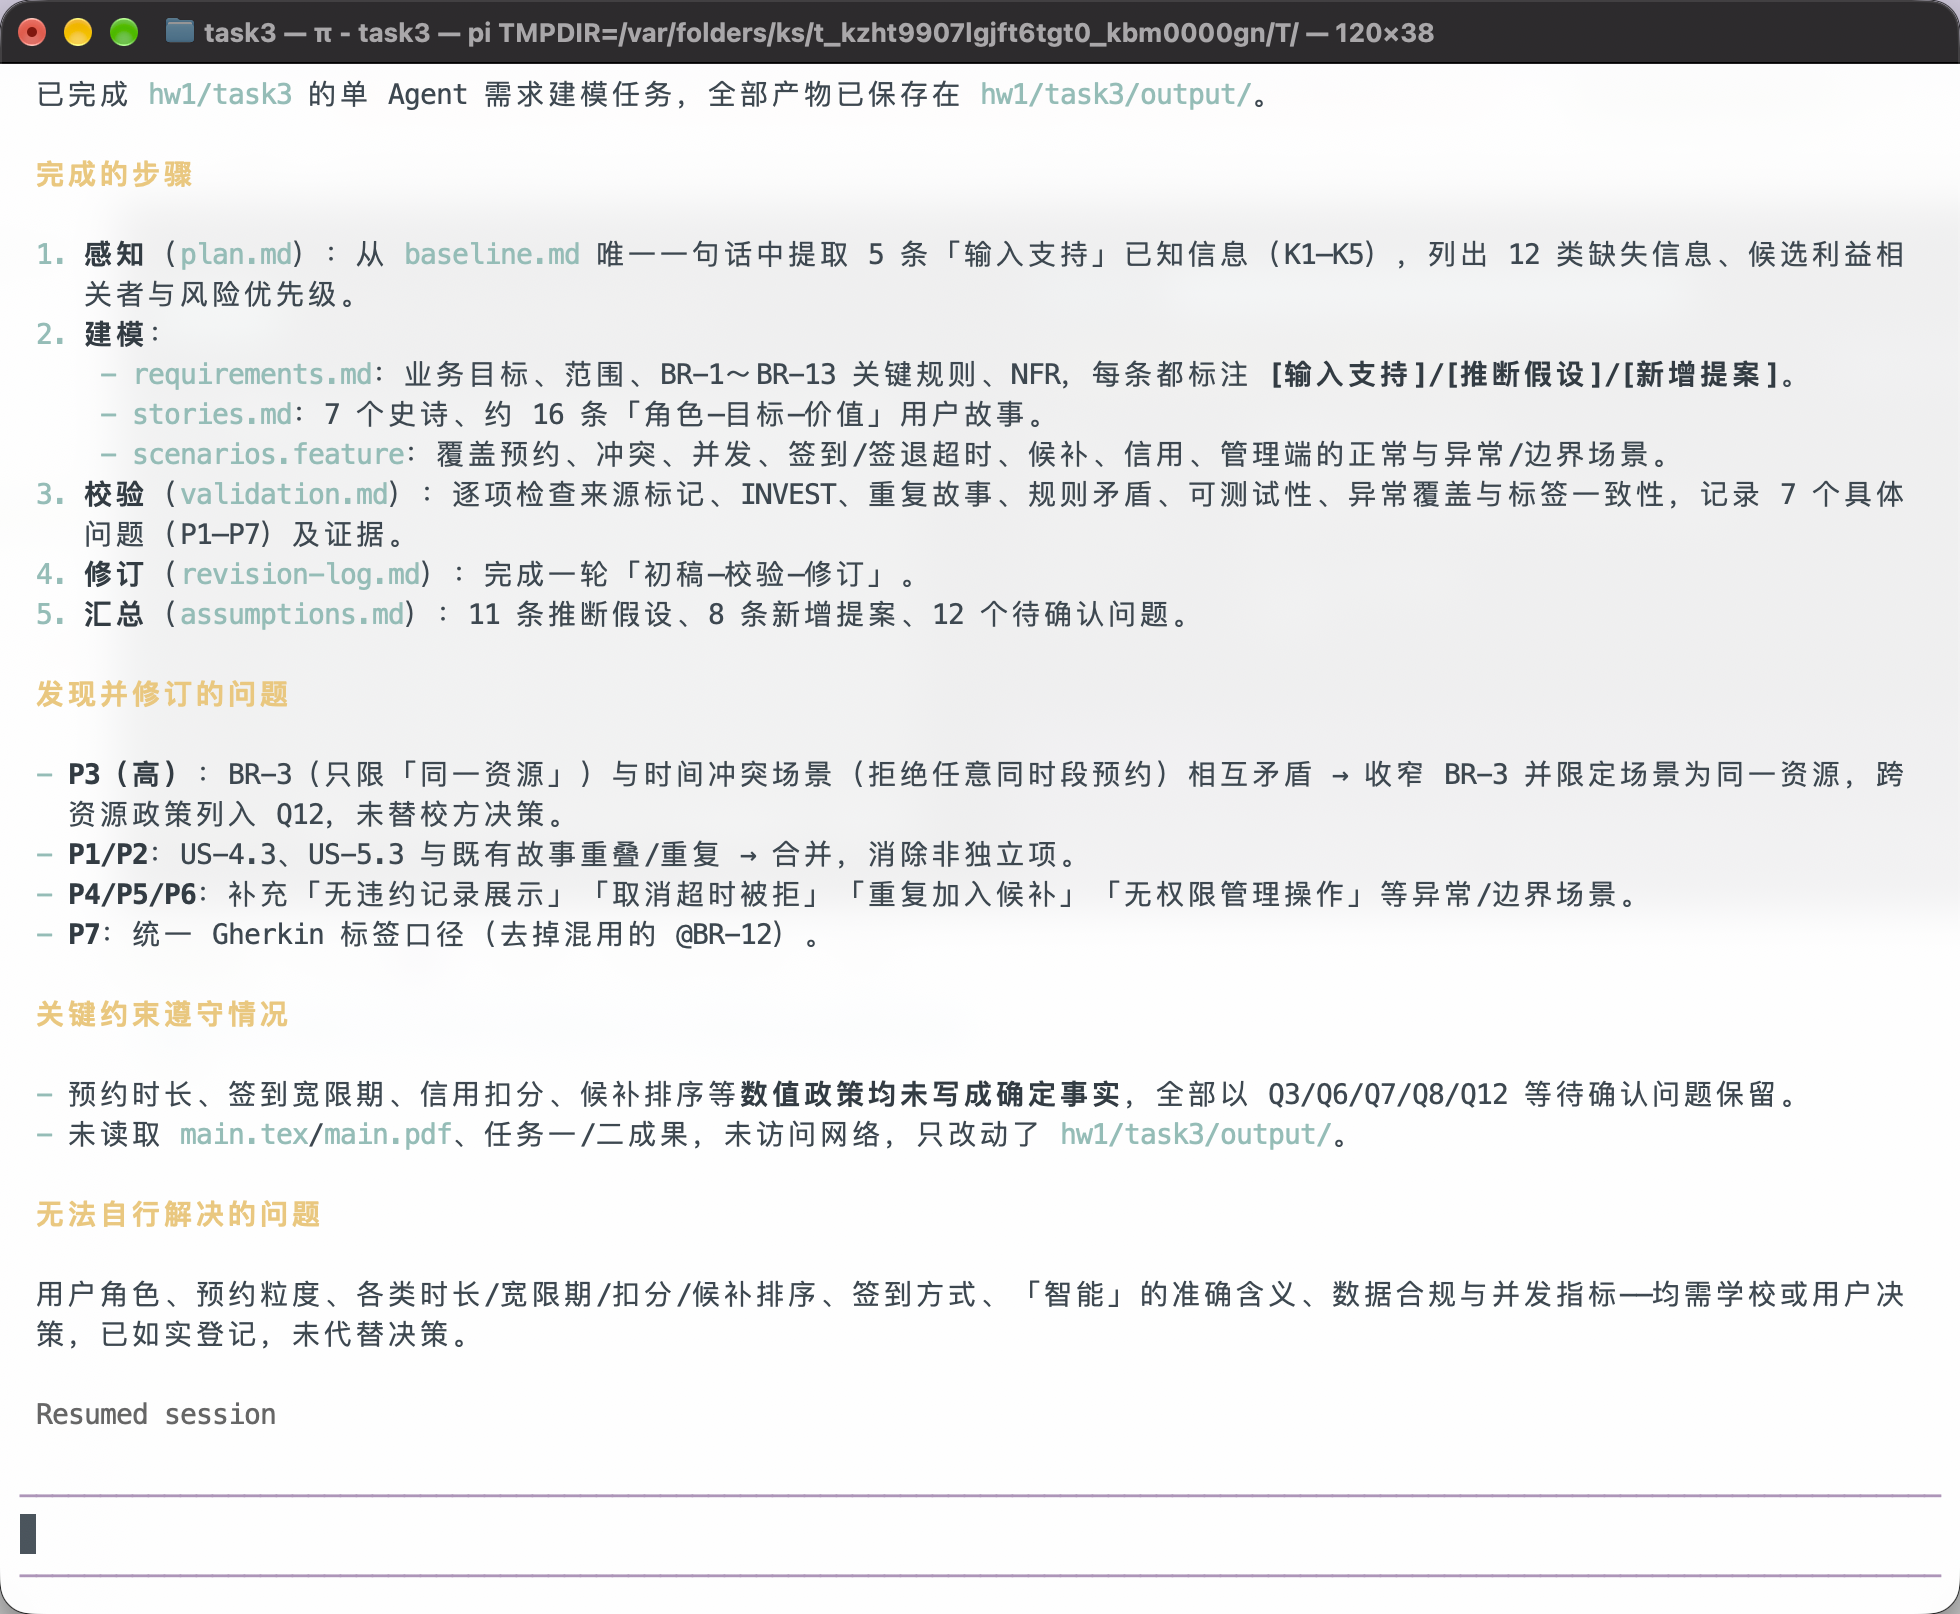
\includegraphics[width=0.9\textwidth]{./figures/agentic_re.png}
  \caption{Agentic SE 需求建模运行情况}
  \label{fig:agentic-re}
\end{figure}

\subsection{Agentic SE需求自治生成的用户故事（节选）}
最终产物按 7 个史诗组织，共保留 18 条用户故事。表~\ref{tab:agentic-story-sample} 节选核心预约、候补、推荐与申诉故事，文字取自修订后的\href{run:task3/output/stories.md}{\texttt{stories.md}}。
其中 US-5.2 已合并重叠的替代方案故事；预约时长、候补排序和“智能”的范围仍待业务方确认。完整故事及关联规则见附录~\ref{app:agentic-stories}，其余产物见附录~\ref{app:agentic-artifacts}。

\begin{longtable}{@{}p{0.12\textwidth}p{0.8\textwidth}@{}}
    \caption{Agentic SE 生成的代表性用户故事}\label{tab:agentic-story-sample} \\
    \toprule
    \textbf{编号} & \textbf{用户故事与确认边界} \\
    \midrule
    US-3.1 & 作为学生，我希望在选定时间段预约可用资源，以便获得确定的自习位置。\par {\small 核心“预约”由输入支持，具体资源与时段规则属推断假设；预约时长与窗口见 Q3。} \\
    \midrule
    US-3.3 & 作为学生，我希望在允许的时限内取消预约，以便行程变化时释放资源。\par {\small 推断假设；可取消时限见 Q4。} \\
    \midrule
    US-5.1 & 作为学生，我希望在目标资源满员时加入候补，以便有空位时能获得使用机会。\par {\small 推断假设；候补排序与通知有效期见 Q8。} \\
    \midrule
    US-5.2 & 作为学生，我希望系统推荐合适的可用资源（当偏好资源不可用时给出替代方案），以便减少选择成本并仍能完成自习安排。\par {\small 推断假设，其中“替代方案”为新增提案；智能范围见 Q9。} \\
    \midrule
    US-6.3 & 作为学生，我希望对误判的违约提出申诉，以便获得人工复核。\par {\small 新增提案；关联 BR-11，误判由管理员人工复核。} \\
    \bottomrule
\end{longtable}

\subsection{Agentic SE需求自治生成的Gherkin格式的BDD场景（节选）}
以下节选四个场景：成功预约展示正常流程；同一资源时间冲突展示 P3 修订后的约束范围；签到超时展示未确认政策的处理方式；重复候补展示 P6 补充的边界场景。
片段沿用最终产物的故事标签，共用其中的 \texttt{Background}。完整的 26 个场景见附录~\ref{app:agentic-bdd}。
Q6、Q7 和 Q12 分别对应签到宽限期、信用政策和跨资源预约限制；这些问题尚未解决，参数及政策确定后仍需细化验收断言。

\begin{framed}
\small
\begin{verbatim}
# language: zh-CN
@校园自习室 @预约系统
Feature: 校园自习室智能预约

  作为校园用户，我希望预约自习室资源并完成签到与签退，
  以便高效、公平地使用自习空间。

  # 说明：场景中的具体时长、宽限期、扣分、候补排序均为占位变量，
  # 不代表已确认政策，需由 Q3/Q6/Q7/Q8 等待确认问题决定。

  Background:
    Given 用户已通过校园身份认证
    And 系统中存在可用自习室「A101」的可预约资源

  @正常 @US-3.1
  Scenario: 成功创建预约
    Given 资源在目标时间段内未被预约
    When 用户选择时间段并提交预约「A101」
    Then 预约创建成功
    And 该资源在目标时间段内标记为已被该用户占用
    And 用户可在「我的预约」中看到这条记录
\end{verbatim}
\end{framed}

\begin{framed}
\small
\begin{verbatim}
  @异常 @US-3.2
  Scenario: 预约与已有预约时间冲突（同一资源）
    Given 用户在同一时间段已有一条针对资源「A101」的有效预约
    When 用户再次提交资源「A101」该时间段的预约
    Then 系统拒绝创建预约
    And 提示用户存在时间冲突
    And 用户的已有预约保持不变

  # 不同资源的同时段预约是否允许，仍由 Q12 确认。
\end{verbatim}
\end{framed}

\begin{framed}
\small
\begin{verbatim}
  @异常 @US-4.1
  Scenario: 超过签到宽限期未签到
    Given 用户存在一条已开始的预约
    And 当前时间已超过签到宽限期
    And 用户尚未签到
    When 系统检测到该超时预约
    Then 预约状态变更为「违约」或「已失效」（依 Q7 政策）
    And 该资源被释放为可预约
    And 按已确认的信用政策处理该用户的记录
\end{verbatim}
\end{framed}

\begin{framed}
\small
\begin{verbatim}
  @边界 @US-5.1
  Scenario: 重复加入同一候补队列
    Given 用户已在某资源的候补队列中
    When 用户再次申请加入同一资源的候补队列
    Then 系统不创建重复的候补记录
    And 用户保持原有候补位置
\end{verbatim}
\end{framed}

\subsection{分析}
本实验中，Agent 工具可以按照程序员定义的流程生成质量更高的需求分析内容。我的理解是：Agent 工具与 LLM 之间的一次交互相当于人与 LLM 的一轮对话，Agent 工具会在每次交互后按预先给定的约束检查结果，如果不符合要求，就带着反馈重新修改内容，直到满足约束或耗尽预算为止。
设本次任务的约束为 $\mathit{constraint}$，目标为 $\mathit{goal}$，用户输入为 $x$，LLM 的输出内容为 $\mathrm{LLM}(x)$，则整个过程可以表示为算法~\ref{alg:agent-loop}。

\begin{algorithm}[htbp]
  \caption{Agent 的“生成—校验—修正”迭代过程}
  \label{alg:agent-loop}
  \begin{algorithmic}[1]
    \Require 用户输入 $x$；约束集合 $C$；最大迭代次数 $N$
    \Ensure 满足约束的输出 $y$；若预算耗尽则返回当前最优结果
    \State $y \gets \mathrm{LLM}(x)$
    \State $n \gets 0$
    \While{$n < N$ 且 $\mathrm{check}(y, C) = \mathrm{false}$}
      \State $d \gets \mathrm{feedback}(y, C)$ \Comment{校验器给出的差异与原因}
      \State $y \gets \mathrm{LLM}(y, d)$ \Comment{把反馈拼回上下文后重新生成}
      \State $n \gets n + 1$
    \EndWhile
    \If{$\mathrm{check}(y, C)$}
      \State \Return $y$
    \Else
      \State \Return $y_{\text{best}}$ \Comment{未收敛，交人工确认}
    \EndIf
  \end{algorithmic}
\end{algorithm}

\section{任务4：总结分析}
表~\ref{tab:modeling-comparison} 对比本次校园自习室预约系统的三种需求建模方式。
人工与 LLM 栏依据任务一及任务二的实际成果；Agentic 栏依据任务三的最终产物和修订日志。
任务三从原始需求独立建模，未读取任务二输出，因此下表区分“相较 LLM 避免的问题”与“Agent 实际修复的自身初稿问题”。
三种方式未统一记录耗时，速度仅作流程层面的定性比较；扩展功能是否应纳入范围，仍需业务方确认。

% 对比维度逐字竖排，与同一行的正文顶部对齐。
\newcommand{\comparisonrowtitle}[1]{\parbox[t]{\linewidth}{\centering\bfseries #1}}
\begingroup
\renewcommand{\thefootnote}{\fnsymbol{footnote}}
\begin{longtable}{@{}p{0.06\textwidth}p{0.28\textwidth}p{0.28\textwidth}p{0.28\textwidth}@{}}
    \caption{传统人工、LLM 增强与 Agentic 自治需求建模对比}\label{tab:modeling-comparison} \\
    \toprule
    \textbf{维度} & \textbf{传统人工建模} & \textbf{LLM增强建模} & \textbf{Agentic自治建模} \\
    \midrule
    \endfirsthead
    \multicolumn{4}{c}{表~\ref{tab:modeling-comparison}（续）} \\
    \toprule
    \textbf{维度} & \textbf{传统人工建模} & \textbf{LLM增强建模} & \textbf{Agentic自治建模} \\
    \midrule
    \endhead
    \bottomrule
    \endlastfoot
    \comparisonrowtitle{速\\度\\与\\工\\作\\量} &
    逐条梳理、编写并人工核对；本次形成 9 条故事、6 个场景，初稿规模较小。
    &
    一次对话生成 20 条故事、29 个场景，扩写快；核实规则与删减扩展仍需人工投入。
    &
    自动执行建模、校验和一轮修订，减少逐项手工整理；多轮调用增加耗时与模型成本。 \\
    \midrule
    \comparisonrowtitle{覆\\盖\\面\\与\\遗\\漏\\与\\补\\全} &
    已覆盖并发抢座、未签到释放和重复教室编号；未写候补、临时闭馆及学生越权管理的验收场景。
    &
    新增候补确认超时、闭馆取消且不扣分、学生访问管理接口被拒等场景；但未覆盖重复加入候补队列。
    &
    修订 P4--P6 补充无违约记录、取消超时、重复候补及无权限管理操作；新增覆盖仍须审核业务合理性。 \\
    \midrule
    \comparisonrowtitle{语\\义\\质\\量\\与\\暂\\离\\与\\释\\放} &
    US-06 同时写“暂时释放座位”和“回来还有座位”，未区分保留占用与向他人开放，存在语义歧义。
    &
    签退场景明确剩余时段可再预约，使“结束使用”更清楚；但没有说明暂离时是否保留座位。
    &
    区分使用中、已完成与超时释放；仍未给出暂离保留规则，不能据此认为所有人工遗漏均已修复。 \\
    \midrule
    \comparisonrowtitle{规\\则\\依\\据\\与\\数\\值\\臆\\定} &
    14:00 开始、14:16 检查的案例未说明宽限期来源；只写受信誉处罚，未明确处罚规则。
    &
    自行规定开始前 30 分钟内取消扣 2 分、爽约扣 5 分、最低信用分 80；这是未确认政策被写成确定规则的风险。
    &
    用参数与待确认问题代替固定政策：Q4 询问取消时限，Q6 询问签到宽限期，Q7 询问信用规则；降低无依据数值进入规格的风险。 \\
    \midrule
    \comparisonrowtitle{一\\致\\性\\与\\候\\补\\排\\序} &
    未建模候补，无法判断先到先得与信用优先如何取舍。
    &
    US-12 写“按候补顺序和信用分”，BDD 却直接通知队列第 1 位；先加入的低信用用户与后加入的高信用用户谁优先，未说明。
    &
    Q8 将排序与通知有效期交业务方确认，场景仅写“按已确认的排序规则”；避免自行选择优先级，但政策尚未解决。 \\
    \midrule
    \comparisonrowtitle{校\\验\\质\\量\\与\\冲\\突\\与\\去\\重} &
    并发场景明确只有一人成功；没有展示系统性的故事去重、规则与场景交叉校验记录。
    &
    并发场景保留一致性约束；“学生不能访问管理员接口”与“权限控制”场景内容重复，仍需整理。
    &
    P1、P2\footnote[1]{P1--P7 是 \texttt{revision-log} 中的问题编号，不是优先级。} 合并重叠故事；P3 修复自身初稿中规则只限制同一资源、场景却拒绝任意同时段预约的范围不一致，跨资源限制保留为 Q12。 \\
    \midrule
    \comparisonrowtitle{可\\追\\溯\\性\\与\\交\\付\\质\\量} &
    表述直观，但规则来源和待确认事项未形成清单，后续变更主要依赖撰写者记忆。
    &
    输出结构完整，但候补、推荐等扩展最初未标来源；任务二分析再人工补充假设追踪表。
    &
    保留来源类别、校验记录与修订日志，便于追踪问题；自检仍可能遗漏，未确认参数与政策须人工补齐后才能作为最终验收依据。 \\
\end{longtable}
\endgroup

上述 Agent 修订可核对\href{run:task3/output/revision-log.md}{修订日志}，政策边界可核对\href{run:task3/output/assumptions.md}{假设与待确认事项}。
本实验显示，LLM 的主要贡献是快速扩展候选需求，Agentic 流程的主要贡献是把生成结果纳入来源标记、校验和修订。
这些改进依赖任务三预先给定的约束，不能仅归因于 Agent 工具本身；自检通过也不等于业务方已经认可需求。
\clearpage
\appendix
\section{Attachment}
以下保留任务二的完整模型输出和任务三的完整用户故事、BDD 场景，并列出任务三产物索引，便于核对正文节选与分析。

\subsection{任务二完整用户故事}\label{app:llm-stories}

\begin{longtable}{@{}p{0.08\textwidth}p{0.75\textwidth}p{0.09\textwidth}@{}}
    \caption{AI生成的完整用户故事列表} \\
    \toprule
    \textbf{编号} & \textbf{用户故事} & \textbf{优先级} \\
    \midrule
    \endfirsthead
    % 续页表头
    \toprule
    \textbf{编号} & \textbf{用户故事} & \textbf{优先级} \\
    \midrule
    \endhead
    \bottomrule
    \endlastfoot
        US-01 & 作为学生，我希望通过校园统一认证登录，以便安全使用预约系统 & P0 \\
        \midrule
        US-02 & 作为学生，我希望查询自习室和座位实时状态，以便选择座位 & P0 \\
        \midrule
        US-03 & 作为学生，我希望按楼层、时间、电源、靠窗筛选座位，以便快速定位 & P0 \\
        \midrule
        US-04 & 作为学生，我希望系统根据偏好、历史、距离推荐座位，以便减少选择成本 & P1 \\
        \midrule
        US-05 & 作为学生，我希望创建预约，以便在指定时间到馆学习 & P0 \\
        \midrule
        US-06 & 作为学生，我希望取消预约，以便计划变化时释放座位 & P0 \\
        \midrule
        US-07 & 作为学生，我希望满座时加入候补，以便有人取消时获得座位 & P1 \\
        \midrule
        US-08 & 作为学生，我希望扫码签到，以便确认到馆并开始使用 & P0 \\
        \midrule
        US-09 & 作为学生，我希望签退或提前释放座位，以便他人使用并积累信用 & P1 \\
        \midrule
        US-10 & 作为学生，我希望查看我的预约、候补和历史，以便管理行程 & P0 \\
        \midrule
        US-11 & 作为系统，我希望自动处理超时未签到，以便释放资源 & P0 \\
        \midrule
        US-12 & 作为系统，我希望按候补顺序和信用分自动分配座位，以便公平高效 & P1 \\
        \midrule
        US-13 & 作为用户，我希望收到预约、签到、候补、闭馆通知，以便及时响应 & P1 \\
        \midrule
        US-14 & 作为管理员，我希望管理自习室、座位、开放时间，以便维护资源 & P0 \\
        \midrule
        US-15 & 作为管理员，我希望配置预约规则和信用规则，以便治理系统 & P0 \\
        \midrule
        US-16 & 作为管理员，我希望处理临时闭馆并批量取消预约，以便应对突发情况 & P1 \\
        \midrule
        US-17 & 作为管理员，我希望查看占用率、违约率、高峰时段报表，以便优化调度 & P1 \\
        \midrule
        US-18 & 作为系统，我希望保证并发预约一致性，以便防止重复预约 & P0 \\
        \midrule
        US-19 & 作为系统，我希望实施权限、安全和审计，以便保护隐私和合规 & P0 \\
        \midrule
        US-20 & 作为系统，我希望通过信用分约束违约行为，以便维护秩序 & P1 \\
\end{longtable}

\subsection{任务二完整Gherkin格式BDD场景}\label{app:llm-bdd}

\begin{framed}
\begin{verbatim}
Feature: 校园统一认证与权限
  作为学生，我希望通过校园统一认证登录，以便安全使用预约系统。

  Scenario: 学生通过校园认证登录
    Given 学生“张三”拥有有效校园账号
    And 用户当前未登录
    When 张三选择“校园统一认证”并完成认证
    Then 系统创建登录会话
    And 跳转到学生首页
    And 显示“自习室查询、我的预约、候补、个人信用”菜单

  Scenario: 未认证用户不能创建预约
    Given 用户未登录
    When 用户请求创建预约
    Then 系统返回“未认证”
    And 不创建任何预约记录

  Scenario: 学生不能访问管理员接口
    Given 学生“张三”已登录
    When 张三请求管理员配置接口
    Then 系统返回“无权限”
    And 记录安全审计日志
\end{verbatim}
\end{framed}

\begin{framed}
\begin{verbatim}
Feature: 自习室与座位查询
  作为学生，我希望查询和筛选实时可用座位，以便选择合适座位。

  Scenario: 查询指定时段可用座位
    Given 学生“张三”已登录
    And 当前时间为 2026-10-10 08:30
    And 自习室“图书馆301”开放时间为 08:00-22:00
    And 座位“A-001”在 09:00-11:00 空闲且非维护
    And 座位“A-002”在 09:00-11:00 已被预约
    When 张三查询 2026-10-10 09:00-11:00 的可用座位
    Then 返回可用座位列表
    And 列表包含“A-001”
    And 列表不包含“A-002”
    And 列表展示座位编号、楼层、电源、靠窗、实时状态

  Scenario: 按设施筛选座位
    Given 学生“张三”已登录
    When 张三筛选“有电源”且“靠窗”的座位
    Then 仅返回同时满足“有电源”和“靠窗”的可用座位
\end{verbatim}
\end{framed}

\begin{framed}
\begin{verbatim}
Feature: 智能座位推荐
  作为学生，我希望系统根据偏好、历史、距离和舒适性推荐座位，以便快速决策。

  Scenario: 基于偏好推荐可用座位
    Given 学生“张三”已登录并设置偏好“靠窗、有电源”
    And 当前时间 2026-10-10 08:30
    And 张三请求 09:00-11:00 的推荐
    And 可用座位包括“A-001（靠窗、有电源）”和“B-002（无电源）”
    When 系统执行智能推荐
    Then 返回最多 3 个推荐座位
    And “A-001”排在“B-002”之前
    And 推荐结果不包含已预约、维护中或不符合开放时间的座位

  Scenario: 无完全匹配时降级推荐
    Given 学生“张三”偏好“靠窗、有电源”
    And 当前没有同时满足两个条件的可用座位
    When 系统执行智能推荐
    Then 返回部分满足条件的次优座位
    And 标注推荐原因和未满足条件
\end{verbatim}
\end{framed}

\begin{framed}
\begin{verbatim}
Feature: 创建预约
  作为学生，我希望在可用时段创建预约，以便到馆学习。

  Scenario: 成功预约空闲座位
    Given 学生“张三”已登录且信用分为 100
    And 自习室“图书馆301”开放时间为 08:00-22:00
    And 座位“A-001”在 2026-10-10 09:00-11:00 未被预约且非维护
    When 张三提交 2026-10-10 09:00-11:00 的预约
    Then 系统创建预约，状态为“已预约”
    And 返回预约编号和签到二维码
    And 该座位在 09:00-11:00 对其他学生不可预约
    And 系统发送预约成功通知

  Scenario: 同一座位同一时段已被预约
    Given 座位“A-001”在 2026-10-10 09:00-11:00 已被李四预约
    When 张三提交同一座位同一时段预约
    Then 系统拒绝预约
    And 提示“该座位时段已被预约”
    And 张三的预约记录不创建

  Scenario Outline: 预约时长校验
    Given 学生“张三”已登录且信用分为 100
    And 座位“A-001”在 2026-10-10 <开始时间> 空闲
    When 张三预约时长 <时长> 分钟
    Then 系统应 <结果>
    Examples:
      | 开始时间 | 时长 | 结果 |
      | 09:00 | 30 | 预约成功 |
      | 09:00 | 240 | 预约成功 |
      | 09:00 | 300 | 拒绝并提示超过最大预约时长 |
\end{verbatim}
\end{framed}

\begin{framed}
\begin{verbatim}
Feature: 取消预约与信用扣减
  作为学生，我希望取消预约，以便计划变化时释放座位。

  Scenario: 开始前 30 分钟免费取消
    Given 学生“张三”已登录且信用分为 100
    And 张三有一个 2026-10-10 09:00 开始的预约
    And 当前时间为 2026-10-10 08:20
    When 张三取消该预约
    Then 取消成功
    And 预约状态变为“已取消”
    And 座位被释放
    And 不扣减信用分

  Scenario: 开始前 30 分钟内取消扣信用
    Given 学生“张三”已登录且信用分为 100
    And 张三有一个 2026-10-10 09:00 开始的预约
    And 当前时间为 2026-10-10 08:45
    When 张三取消该预约
    Then 取消成功
    And 扣减 2 点信用分
    And 记录取消原因和时间
\end{verbatim}
\end{framed}

\begin{framed}
\begin{verbatim}
Feature: 候补队列
  作为学生，我希望在满座时加入候补，以便有人取消时自动获得座位。

  Scenario: 加入候补
    Given 学生“张三”已登录且信用分为 100
    And 座位“A-001”在 2026-10-10 09:00-11:00 已被预约
    When 张三申请加入该时段的候补
    Then 系统创建候补记录，状态为“候补中”
    And 返回候补顺序号
    And 系统发送候补加入成功通知

  Scenario: 候补自动分配与确认
    Given 学生“张三”在候补队列第 1 位
    And 学生“李四”的预约在 2026-10-10 09:00-11:00 被取消
    When 系统释放座位“A-001”
    Then 系统向张三发送候补确认通知
    And 张三有 10 分钟确认时间
    When 张三在 10 分钟内确认
    Then 系统为张三创建预约
    And 从候补队列移除张三
    And 通知其他候补者继续等待

  Scenario: 候补确认超时顺延
    Given 学生“张三”收到候补确认通知
    And 张三在 10 分钟内未确认
    When 确认时间超时
    Then 系统取消张三的候补确认资格
    And 按顺序通知下一位候补者
\end{verbatim}
\end{framed}

\begin{framed}
\begin{verbatim}
Feature: 签到、签退与超时处理
  作为学生/系统，我希望完成签到签退并自动释放超时资源。

  Scenario: 扫码签到成功
    Given 学生“张三”已登录
    And 张三有 2026-10-10 09:00-11:00 座位“A-001”的预约
    And 当前时间为 2026-10-10 08:55
    When 张三扫描座位二维码签到
    Then 签到成功
    And 预约状态变为“已签到”
    And 记录签到时间
    And 系统开始计时

  Scenario: 超时未签到自动取消
    Given 学生“张三”有 2026-10-10 09:00 开始的预约
    And 当前时间已到 2026-10-10 09:15
    And 张三未签到
    When 系统执行超时检查
    Then 预约状态变为“爽约”
    And 释放座位
    And 扣减张三 5 点信用分
    And 发送违约通知

  Scenario: 签退释放座位
    Given 学生“张三”已签到座位“A-001”
    And 当前时间为 2026-10-10 10:30
    When 张三执行签退
    Then 预约状态变为“已完成”
    And 座位从 10:30 起释放
    And 记录实际使用时长
\end{verbatim}
\end{framed}

\begin{framed}
\begin{verbatim}
Feature: 信用分管理
  作为系统，我希望通过信用分约束违约行为。

  Scenario Outline: 信用分限制预约
    Given 学生“张三”已登录，信用分为 <信用分>
    And 系统预约最低信用分为 80
    When 张三提交预约
    Then 系统应 <结果>
    Examples:
      | 信用分 | 结果 |
      | 100 | 允许预约 |
      | 80 | 允许预约 |
      | 79 | 拒绝预约并提示信用分不足 |
\end{verbatim}
\end{framed}

\begin{framed}
\begin{verbatim}
Feature: 通知
  作为学生/管理员，我希望收到关键事件通知。

  Scenario: 预约成功通知
    Given 学生“张三”创建预约成功
    When 系统完成预约创建
    Then 发送站内信/微信/邮件通知
    And 通知包含时间、地点、座位号、签到提醒

  Scenario: 签到提醒
    Given 张三有 09:00 开始的预约
    And 当前时间为 08:45
    When 系统执行提醒任务
    Then 向张三发送签到提醒
    And 提醒包含签到二维码入口和超时规则

  Scenario: 临时闭馆通知
    Given 管理员将“图书馆301”在 2026-10-10 14:00-18:00 设为临时闭馆
    When 系统处理受影响预约
    Then 自动取消相关预约
    And 不扣减学生信用分
    And 向受影响学生发送闭馆和取消通知
\end{verbatim}
\end{framed}

\begin{framed}
\begin{verbatim}
Feature: 管理员资源与规则管理
  作为管理员，我希望管理自习室、座位、开放时间和规则。

  Scenario: 创建自习室和座位
    Given 管理员已登录
    When 管理员创建自习室“图书馆301”，开放时间 08:00-22:00
    And 批量导入座位“A-001”至“A-100”
    Then 保存成功
    And 学生可查询到这些座位

  Scenario: 配置预约规则
    Given 管理员已登录
    When 管理员设置最大预约时长 240 分钟、提前预约 7 天、签到宽限 15 分钟
    Then 保存成功
    And 新规则立即对后续预约生效
\end{verbatim}
\end{framed}

\begin{framed}
\begin{verbatim}
Feature: 报表与监控
  作为管理员，我希望查看占用率和违约报表。

  Scenario: 查看占用率
    Given 管理员已登录
    And 2026-10-10 图书馆301有 100 个座位
    And 该日 09:00-11:00 有 80 个预约
    When 管理员查询该时段占用率
    Then 显示占用率为 80%
    And 显示各楼层/时段趋势

  Scenario: 导出报表
    Given 管理员已登录并查询到报表数据
    When 管理员选择导出 CSV
    Then 系统生成 CSV 文件
    And 文件包含日期、自习室、时段、预约数、占用率、违约数
\end{verbatim}
\end{framed}

\begin{framed}
\begin{verbatim}
Feature: 并发一致性与安全审计
  作为系统，我希望防止重复预约并保护数据安全。

  Scenario: 两个学生同时预约同一座位同一时段
    Given 座位“A-001”在 2026-10-10 09:00-11:00 空闲
    And 学生“张三”和“李四”同时提交该座位该时段预约
    When 系统处理并发请求
    Then 仅一个预约成功
    And 另一个返回“座位已被预约”
    And 数据库中不存在同一座位同一时段的重复有效预约

  Scenario: 权限控制
    Given 学生“张三”已登录
    When 张三请求管理员配置接口
    Then 系统返回“无权限”
    And 记录安全审计日志

  Scenario: 审计日志
    Given 管理员修改了预约规则
    When 系统保存修改
    Then 记录操作人、时间、修改前后内容
    And 日志不可被普通用户修改
\end{verbatim}
\end{framed}


\clearpage
\subsection{任务三产物索引}\label{app:agentic-artifacts}
任务三依据\href{run:task3/baseline.md}{原始需求}与\href{run:task3/agent-task.md}{建模任务约束}独立生成。下表列出完整产物；随后嵌入全部用户故事与 BDD 场景。来源类别、关联规则与待确认事项均按最终文件保留，不把候选政策视为已确认需求。

\begin{longtable}{@{}p{0.3\textwidth}p{0.62\textwidth}@{}}
    \caption{Agentic SE 完整产物索引} \\
    \toprule
    \textbf{产物} & \textbf{内容与用途} \\
    \midrule
    \endfirsthead
    \toprule
    \textbf{产物} & \textbf{内容与用途} \\
    \midrule
    \endhead
    \bottomrule
    \endlastfoot
    \href{run:task3/output/plan.md}{\texttt{plan.md}} & 感知结果、缺失信息、建模步骤及风险规划。 \\
    \midrule
    \href{run:task3/output/requirements.md}{\texttt{requirements.md}} & 业务目标、系统范围、BR-1 至 BR-13 业务规则及非功能需求。 \\
    \midrule
    \href{run:task3/output/stories.md}{\texttt{stories.md}} & 7 个史诗、18 条最终用户故事及来源、关联规则和修订说明。 \\
    \midrule
    \href{run:task3/output/scenarios.feature}{\texttt{scenarios.feature}} & 包含公共前置条件、故事标签、26 个正常、异常及边界场景的原始文本。 \\
    \midrule
    \href{run:task3/output/validation.md}{\texttt{validation.md}} & 来源、INVEST、重复故事、规则矛盾及场景覆盖的检查证据。 \\
    \midrule
    \href{run:task3/output/revision-log.md}{\texttt{revision-log.md}} & P1 至 P7 的问题、实际修改及仍待人工确认的事项。 \\
    \midrule
    \href{run:task3/output/assumptions.md}{\texttt{assumptions.md}} & 推断假设、新增提案，以及 Q1 至 Q12 待确认问题的完整清单。 \\
    \midrule
    \href{run:task3/output/session.pdf}{\texttt{session.pdf}} & 独立提供的完整 Agent 运行记录。 \\
\end{longtable}

\subsection{任务三完整用户故事}\label{app:agentic-stories}

\subsubsection{EP-1 身份与权限}
来源类别：[推断假设]。

\begin{longtable}{@{}p{0.12\textwidth}p{0.8\textwidth}@{}}
    \toprule
    \textbf{编号} & \textbf{用户故事与关联信息} \\
    \midrule
    \endfirsthead
    \toprule
    \textbf{编号} & \textbf{用户故事与关联信息} \\
    \midrule
    \endhead
    \bottomrule
    \endlastfoot
    US-1.1 & \textbf{登录}\par 作为学生，我希望用校园身份登录，以便安全地使用预约服务。\par {\small 关联：BR-1、BR-12。验收指向scenarios.feature 中「登录后才能预约」。} \\
    \midrule
    US-1.2 & \textbf{权限隔离}\par 作为用户，我希望只能看到与操作自己的预约，以便我的信息不被他人查看。\par {\small 关联：BR-12。} \\
\end{longtable}

\subsubsection{EP-2 自习室资源浏览与检索}
来源类别：[推断假设]。

\begin{longtable}{@{}p{0.12\textwidth}p{0.8\textwidth}@{}}
    \toprule
    \textbf{编号} & \textbf{用户故事与关联信息} \\
    \midrule
    \endfirsthead
    \toprule
    \textbf{编号} & \textbf{用户故事与关联信息} \\
    \midrule
    \endhead
    \bottomrule
    \endlastfoot
    US-2.1 & \textbf{浏览资源}\par 作为学生，我希望查看自习室及其可用资源与空闲时段，以便决定去哪自习。\par {\small 关联：BR-2。资源粒度见 Q2。} \\
    \midrule
    US-2.2 & \textbf{检索与筛选}\par 作为学生，我希望按地点、时间、容量等条件筛选，以便快速找到合适的自习室。\par {\small 关联：BR-2、NFR-4。筛选维度为 [新增提案]。} \\
\end{longtable}

\subsubsection{EP-3 预约创建与管理}
来源类别：[推断假设] + [输入支持]（核心词「预约」）。

\begin{longtable}{@{}p{0.12\textwidth}p{0.8\textwidth}@{}}
    \toprule
    \textbf{编号} & \textbf{用户故事与关联信息} \\
    \midrule
    \endfirsthead
    \toprule
    \textbf{编号} & \textbf{用户故事与关联信息} \\
    \midrule
    \endhead
    \bottomrule
    \endlastfoot
    US-3.1 & \textbf{创建预约}\par 作为学生，我希望在选定时间段预约可用资源，以便获得确定的自习位置。\par {\small 关联：BR-2、BR-3、NFR-2。时长与窗口见 Q3。} \\
    \midrule
    US-3.2 & \textbf{避免冲突}\par 作为学生，我希望系统在我重复预约冲突时段时给出提示，以便避免无效预约。\par {\small 关联：BR-3。} \\
    \midrule
    US-3.3 & \textbf{取消预约}\par 作为学生，我希望在允许的时限内取消预约，以便行程变化时释放资源。\par {\small 关联：BR-4。时限见 Q4。} \\
    \midrule
    US-3.4 & \textbf{查看我的预约}\par 作为学生，我希望查看自己的当前与历史预约，以便管理行程。\par {\small 关联：BR-12。} \\
\end{longtable}

\subsubsection{EP-4 签到、签退与资源释放}
来源类别：[推断假设]。

\begin{longtable}{@{}p{0.12\textwidth}p{0.8\textwidth}@{}}
    \toprule
    \textbf{编号} & \textbf{用户故事与关联信息} \\
    \midrule
    \endfirsthead
    \toprule
    \textbf{编号} & \textbf{用户故事与关联信息} \\
    \midrule
    \endhead
    \bottomrule
    \endlastfoot
    US-4.1 & \textbf{签到}\par 作为学生，我希望到馆后完成签到，以便确认我实际使用该座位。\par {\small 关联：BR-5。方式与宽限期见 Q5、Q6。} \\
    \midrule
    US-4.2 & \textbf{签退}\par 作为学生，我希望使用结束后签退，以便资源及时释放给他人。\par {\small 关联：BR-6。} \\
\end{longtable}

\noindent 修订说明（校验 P1）：原 US-4.3「超时处理」描述的是系统行为而非学生目标，且与 US-4.1/US-4.2 重叠，已并入两条故事的异常场景（见 scenarios.feature 的「超过签到宽限期未签到」「未签退导致超时占用」），不再单列故事。

\subsubsection{EP-5 候补与智能推荐}
来源类别：[推断假设]。

\begin{longtable}{@{}p{0.12\textwidth}p{0.8\textwidth}@{}}
    \toprule
    \textbf{编号} & \textbf{用户故事与关联信息} \\
    \midrule
    \endfirsthead
    \toprule
    \textbf{编号} & \textbf{用户故事与关联信息} \\
    \midrule
    \endhead
    \bottomrule
    \endlastfoot
    US-5.1 & \textbf{候补}\par 作为学生，我希望在目标资源满员时加入候补，以便有空位时能获得使用机会。\par {\small 关联：BR-8。排序见 Q8。} \\
    \midrule
    US-5.2 & \textbf{智能推荐}\par 作为学生，我希望系统推荐合适的可用资源（当偏好资源不可用时给出替代方案），以便减少选择成本并仍能完成自习安排。\par {\small 关联：BR-9。含义见 Q9。[推断假设]，其中「替代方案」为 [新增提案]。}\par {\small 修订说明（校验 P2）：原 US-5.3「冲突消解」与 US-5.2 边界模糊、行为重合，已合并入本故事，不再单列。} \\
\end{longtable}

\subsubsection{EP-6 违约与信用}
来源类别：[推断假设]／[新增提案]。

\begin{longtable}{@{}p{0.12\textwidth}p{0.8\textwidth}@{}}
    \toprule
    \textbf{编号} & \textbf{用户故事与关联信息} \\
    \midrule
    \endfirsthead
    \toprule
    \textbf{编号} & \textbf{用户故事与关联信息} \\
    \midrule
    \endhead
    \bottomrule
    \endlastfoot
    US-6.1 & \textbf{违约提示}\par 作为学生，我希望在可能违约前收到提醒，以便避免被记录违约。\par {\small 关联：BR-7。提醒时机为 [新增提案]，见 Q7。} \\
    \midrule
    US-6.2 & \textbf{信用查询}\par 作为学生，我希望查看自己的信用/违约记录，以便了解自身状态。\par {\small 关联：BR-7。[新增提案]。} \\
    \midrule
    US-6.3 & \textbf{申诉}\par 作为学生，我希望对误判的违约提出申诉，以便获得人工复核。\par {\small 关联：BR-11。[新增提案]。} \\
\end{longtable}

\subsubsection{EP-7 管理端运维与统计}
来源类别：[新增提案]。

\begin{longtable}{@{}p{0.12\textwidth}p{0.8\textwidth}@{}}
    \toprule
    \textbf{编号} & \textbf{用户故事与关联信息} \\
    \midrule
    \endfirsthead
    \toprule
    \textbf{编号} & \textbf{用户故事与关联信息} \\
    \midrule
    \endhead
    \bottomrule
    \endlastfoot
    US-7.1 & \textbf{资源维护}\par 作为管理员，我希望创建、修改、停用自习室与资源，以便保持资源信息准确。\par {\small 关联：BR-10。[新增提案]。} \\
    \midrule
    US-7.2 & \textbf{处置违规}\par 作为管理员，我希望查看并处置违规与申诉，以便维持秩序与公平。\par {\small 关联：BR-11。[新增提案]。} \\
    \midrule
    US-7.3 & \textbf{统计报表}\par 作为管理员，我希望查看使用率与违约统计，以便优化资源配置。\par {\small 关联：G2、BR-11。[新增提案]。} \\
\end{longtable}

\subsection{任务三完整Gherkin格式BDD场景}\label{app:agentic-bdd}
以下收录最终 \texttt{scenarios.feature} 的全部内容，按原有顺序分块排版，共用同一 \texttt{Feature} 与 \texttt{Background}。保留原始标签、注释和待确认政策；长行仅作排版换行，原始文件见\href{run:task3/output/scenarios.feature}{\texttt{scenarios.feature}}。

\begin{framed}
\small
\begin{verbatim}
# language: zh-CN
@校园自习室 @预约系统
Feature: 校园自习室智能预约

  作为校园用户，我希望预约自习室资源并完成签到与签退，
  以便高效、公平地使用自习空间。

  # 说明：场景中的具体时长、宽限期、扣分、候补排序均为占位变量，
  # 不代表已确认政策，需由 Q3/Q6/Q7/Q8 等待确认问题决定。

  Background:
    Given 用户已通过校园身份认证
    And 系统中存在可用自习室「A101」的可预约资源

  # ---------------- EP-3 预约创建与管理（正常流程） ----------------
\end{verbatim}
\end{framed}

\begin{framed}
\small
\begin{verbatim}
  @正常 @US-3.1
  Scenario: 成功创建预约
    Given 资源在目标时间段内未被预约
    When 用户选择时间段并提交预约「A101」
    Then 预约创建成功
    And 该资源在目标时间段内标记为已被该用户占用
    And 用户可在「我的预约」中看到这条记录
\end{verbatim}
\end{framed}

\begin{framed}
\small
\begin{verbatim}
  @正常 @US-3.1 @US-5.2
  Scenario: 用户不清楚去哪时获得智能推荐
    Given 用户在目标时间段内没有已存在的预约
    When 用户请求推荐可用的自习室资源
    Then 系统返回一个或多个可用资源建议
    And 每条建议包含地点与可用时间段信息
\end{verbatim}
\end{framed}

\begin{framed}
\small
\begin{verbatim}
  @正常 @US-3.3
  Scenario: 在允许时限内取消预约
    Given 用户存在一条未来时段的预约
    And 当前时间处于可取消时限内
    When 用户取消该预约
    Then 预约状态变更为「已取消」
    And 该资源在目标时间段内恢复为可预约
\end{verbatim}
\end{framed}

\begin{framed}
\small
\begin{verbatim}
  @正常 @US-3.4
  Scenario: 查看我的预约
    Given 用户存在若干当前与历史预约
    When 用户打开「我的预约」
    Then 系统仅展示属于该用户的预约记录

  # ---------------- 预约异常与边界 ----------------
\end{verbatim}
\end{framed}

\begin{framed}
\small
\begin{verbatim}
  @异常 @US-3.2
  Scenario: 预约与已有预约时间冲突（同一资源）
    Given 用户在同一时间段已有一条针对资源「A101」的有效预约
    When 用户再次提交资源「A101」该时间段的预约
    Then 系统拒绝创建预约
    And 提示用户存在时间冲突
    And 用户的已有预约保持不变

  # 待确认：同一用户在同一时段预约**不同资源**是否允许由 Q12 决定，
  # 因此不写死对应场景，避免替校方决策。
\end{verbatim}
\end{framed}

\begin{framed}
\small
\begin{verbatim}
  @异常 @US-3.1
  Scenario: 预约已被他人占用的资源
    Given 资源在目标时间段已被其他用户预约
    When 用户提交该资源在该时间段的预约
    Then 系统拒绝创建预约
    And 提示该资源在目标时间段不可用
\end{verbatim}
\end{framed}

\begin{framed}
\small
\begin{verbatim}
  @异常 @US-3.1
  Scenario: 并发抢同一资源时只允许一人成功
    Given 资源在目标时间段内空闲
    And 两名用户几乎同时提交对该资源的同一时间段预约
    When 系统处理这两个并发请求
    Then 至多一个预约创建成功
    And 另一个请求被拒绝并提示资源不可用
\end{verbatim}
\end{framed}

\begin{framed}
\small
\begin{verbatim}
  @边界 @US-3.1
  Scenario: 超出允许预约时间窗口
    Given 存在「允许提前预约窗口」参数
    When 用户选择超出该窗口的时间段提交预约
    Then 系统拒绝创建预约
    And 提示该时间超出可预约范围
\end{verbatim}
\end{framed}

\begin{framed}
\small
\begin{verbatim}
  @正常 @US-1.2
  Scenario: 用户访问他人预约
    Given 用户 A 存在一条预约
    When 用户 B 尝试查看或修改用户 A 的预约
    Then 系统拒绝该操作
    And 不泄露用户 A 的预约详情

  # ---------------- EP-4 签到与签退 ----------------
\end{verbatim}
\end{framed}

\begin{framed}
\small
\begin{verbatim}
  @正常 @US-4.1
  Scenario: 按时签到
    Given 用户存在一条即将开始的预约
    And 当前时间处于签到宽限期内
    When 用户完成签到
    Then 该预约状态变更为「使用中」
\end{verbatim}
\end{framed}

\begin{framed}
\small
\begin{verbatim}
  @异常 @US-4.1
  Scenario: 超过签到宽限期未签到
    Given 用户存在一条已开始的预约
    And 当前时间已超过签到宽限期
    And 用户尚未签到
    When 系统检测到该超时预约
    Then 预约状态变更为「违约」或「已失效」（依 Q7 政策）
    And 该资源被释放为可预约
    And 按已确认的信用政策处理该用户的记录
\end{verbatim}
\end{framed}

\begin{framed}
\small
\begin{verbatim}
  @正常 @US-4.2
  Scenario: 使用结束后签退
    Given 用户存在一条状态为「使用中」的预约
    When 用户完成签退
    Then 预约状态变更为「已完成」
    And 该资源在剩余时间段内释放为可预约
\end{verbatim}
\end{framed}

\begin{framed}
\small
\begin{verbatim}
  @异常 @US-4.2
  Scenario: 未签退导致超时占用
    Given 用户存在一条状态为「使用中」的预约
    And 已超过预约结束时间
    And 用户未签退
    When 系统检测到超时占用
    Then 系统结束该预约并释放资源
    And 按政策记录相应的违约处理

  # ---------------- EP-5 候补 ----------------
\end{verbatim}
\end{framed}

\begin{framed}
\small
\begin{verbatim}
  @正常 @US-5.1
  Scenario: 满员时进入候补
    Given 目标资源在目标时间段已满
    When 用户选择加入候补队列
    Then 用户被加入该资源的候补列表
    And 系统告知用户候补位置或通知方式
\end{verbatim}
\end{framed}

\begin{framed}
\small
\begin{verbatim}
  @正常 @US-5.1
  Scenario: 候补获得释放的资源
    Given 用户在某资源的候补队列中
    And 该资源对应时段因取消或违约被释放
    When 系统按候补规则分配该资源
    Then 系统按已确认的排序规则通知候补用户
    And 被通知用户可在有效期内确认占用
\end{verbatim}
\end{framed}

\begin{framed}
\small
\begin{verbatim}
  @边界 @US-5.1
  Scenario: 候补通知确认超时
    Given 用户已收到候补可用通知
    And 用户在有效确认时间内未确认
    When 系统检测到确认超时
    Then 系统将该机会顺延给下一位候补用户
\end{verbatim}
\end{framed}

\begin{framed}
\small
\begin{verbatim}
  @异常 @US-3.3
  Scenario: 超出可取消时限后被拒绝取消
    Given 用户存在一条未来时段的预约
    And 当前时间已超出可取消时限
    When 用户尝试取消该预约
    Then 系统拒绝取消
    And 预约状态保持有效
\end{verbatim}
\end{framed}

\begin{framed}
\small
\begin{verbatim}
  @边界 @US-5.1
  Scenario: 重复加入同一候补队列
    Given 用户已在某资源的候补队列中
    When 用户再次申请加入同一资源的候补队列
    Then 系统不创建重复的候补记录
    And 用户保持原有候补位置
\end{verbatim}
\end{framed}

\begin{framed}
\small
\begin{verbatim}
  @异常 @US-7.1
  Scenario: 无管理权限的用户执行管理操作
    Given 用户不具备管理员权限
    When 用户尝试创建或修改自习室资源
    Then 系统拒绝该操作
    And 不产生任何资源变更

  # ---------------- EP-6 违约与信用 ----------------
\end{verbatim}
\end{framed}

\begin{framed}
\small
\begin{verbatim}
  @正常 @US-6.1
  Scenario: 临近预约开始时收到提醒
    Given 用户存在一条即将开始的预约
    When 到达提醒时间点
    Then 系统向用户发送提醒
    And 提醒包含签到时间要求
\end{verbatim}
\end{framed}

\begin{framed}
\small
\begin{verbatim}
  @正常 @US-6.2
  Scenario: 查询自身信用记录
    Given 用户曾发生违约
    When 用户查看信用/违约记录
    Then 系统仅展示该用户的记录与状态
\end{verbatim}
\end{framed}

\begin{framed}
\small
\begin{verbatim}
  @正常 @US-6.2
  Scenario: 无违约记录时的信用展示
    Given 用户没有任何违约记录
    When 用户查看信用/违约记录
    Then 系统展示空记录状态或正常信用状态
    And 不展示其他用户的记录
\end{verbatim}
\end{framed}

\begin{framed}
\small
\begin{verbatim}
  @正常 @US-6.3
  Scenario: 提交违约申诉
    Given 用户认为某条违约记录有误
    When 用户对该记录提交申诉
    Then 系统创建待处理申诉
    And 交给管理员复核

  # ---------------- EP-7 管理端 ----------------
\end{verbatim}
\end{framed}

\begin{framed}
\small
\begin{verbatim}
  @正常 @US-7.1
  Scenario: 管理员维护自习室资源
    Given 管理员已登录并具备管理权限
    When 管理员创建或修改自习室「A101」的资源信息
    Then 变更被保存
    And 用户端可见最新的资源信息
\end{verbatim}
\end{framed}

\begin{framed}
\small
\begin{verbatim}
  @异常 @US-7.1
  Scenario: 停用存在未来预约的资源
    Given 某资源存在未来有效预约
    When 管理员停用该资源
    Then 系统提示受影响的预约
    And 按已确认政策处理这些预约（如通知或改约）
\end{verbatim}
\end{framed}

\begin{framed}
\small
\begin{verbatim}
  @正常 @US-7.3
  Scenario: 管理员查看使用统计
    Given 管理员已登录并具备管理权限
    When 管理员查看某自习室的使用率报表
    Then 系统展示该资源在所选周期内的使用统计
\end{verbatim}
\end{framed}

\end{document}
